\chapter{Ergebnisse}
%Sandra
\Autor{Sandra Schröder}
\begin{itemize}
	\item Vergleich der Algorithmen
	\item Anhand der Kriterien: QUELLE!!!
	\begin{itemize}
		\item Erhaltung der Topologie
		\item Pixelkonnektivität
		\item Zentriert
		\item 1 Pixel breit
		\item Robustheit
	\end{itemize}
	\item Vergleich anhand von Screenshots
	\item Echtzeitfähigkeit -> Messungen machen -> Vergleich
	\item Verbesserung des Skeletts (Distanztransformation) mit Breitensuche um Pixelkonnektivität zu erreichen -> Weitere Verbesserungen?
\end{itemize}
\section{Vergleich der Algorithmen}
Screenshots und Laufzeitmessungen
\section{Verbesserung der Skelettqualität}
Das Skelett, welches mit der Methode der Distanztransformation bestimmt wurde, weist Lücken zwischen den Skelettteilen auf. Die Ursache sind der Gradientenbetrag, der für die Extraktion der Skelettlinie berechnet wurde und die Segmentierung des Gradientenbildes. Abbildung \ref{fig:hand-skelett} zeigt ein Beispiel dazu. Abbildung (a) ist das Originalbild mit dem Objekt, von dem das Skelett, wie in Abbildung (c) zu sehen, bestimmt wurde. Da der Algorithmus auf der Grundlage von Bildern arbeitet, bei denen das Objekt und der Hintergrund schwarz markiert sind,
wurde das Bild zuvor invertiert. Abbildung (b) zeigt die Distance Map des Originalbildes. Abbildung (d) ist das Gradientenbild der Distance Map. Das Gradientenbild wurde mit einem empirisch gewählten Schwellwert segmentiert, um anschließend die Skelettlinie zu extrahieren. Dadurch werden Linien im Gradientenbild, die einen kleineren Grauwert als der Schwellwert besitzen, eliminiert. \\
In den folgenden Abschnitten werden Methoden zur Verbesserung des Skeletts vorgestellt. Dies umfasst zum einen die Herstellung Pixelkonnektivität beziehungsweise dem Füllen der Lücken zwischen den Skelettlinien. Zum anderen ist es wünschenswert, dass die Skelettlinie des Objektes nicht breiter als ein Pixel ist. Zuerst wurden markante Punkte auf dem Skelett bestimmt. Diese wurden
genutzt, um mittels Breitensuche und Tiefensuche Pfade zwischen ihnen zu finden und sie zu verbinden. Punkte werden miteinander
verbunden, wenn sie nah genug beieinander sind. Das Ergebnis ist ein Skelett
zusammenhängenden Skelettlinien. Die genaue Umsetzung der Algorithmen wird in den Abschnitten \ref{subsec:breitesuche} und \ref{subsec:tiefensuche} beschrieben.\\
Breiten -und Tiefensuche liefern aufgrund ihrer algorithmischen Eigenschaften jeweils unterschiedliche Ergebnisse. Die Unterschiede werden gezeigt und es wird diskutiert, inwieweit sich die Verfahren mit der Kinect in Echtzeit anwenden lassen. 
\begin{figure}
\centering
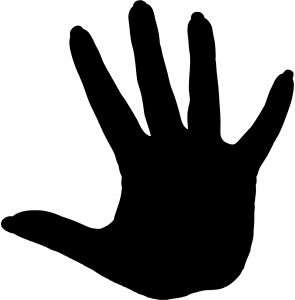
\includegraphics[width=1.0\linewidth]{./fig/hand}
\caption{Bestimmung des Skelett mittels Distanztransformation. (a) Originalbild (b) Distance Map (c) Gradientenbild (d) Skelett}
\label{fig:hand-skelett}
\end{figure}
\newpage
\subsection{Berechnung von Features auf dem Skelett}
Die Bildverarbeitungsbibliothek \emph{OpenCV} bietet Funktionen zur Bestimmung von markanten Punkten, sogenannten \emph{Features},
in einem Bild. Die Funktion \texttt{goodFeaturesToTrack} bestimmt die am stärkesten auftretenden Ecken in einem Bild oder Bildausschnitt nach einem Algorithmus von \cite{goodfeatures}. Mittels eines Qualitätsmaßes wird entschieden, ob die Stärke einer
Ecke an einem bestimmten Pixel ausreicht, um in die Featuremenge aufgenommen zu werden. Für die
Funktion können der Wert des Qualitätsmaßes, den eine Ecke erfüllen muss, die Anzahl der Ecken, die gefunden werden sollen und die
minimale Distanz zwischen den stärksten Ecken übergeben werden.\\
Die Qualität einer Ecke wird anhand von Eigenwerten bestimmt. Die Eigenwerte beziehen sich dabei auf 
die Kovarianzmatrix von Ableitungen einer festgelegten Umgebung eines Pixels. Es wird minimale Eigenwert
für die Eckendetektion weiterverwendet. Ist der minimale Eigenwert einer Ecke kleiner als das gewünschte
Qualitätsmaß, wird diese Ecke verworfen. Die verbleibenden Ecken werden nach ihrer Qualität absteigend sortiert. Anschließend wird überprüft, ob es in der spezifizierten Distanz Ecken gibt, die stärker sind. 
\begin{figure}[h]
\centering
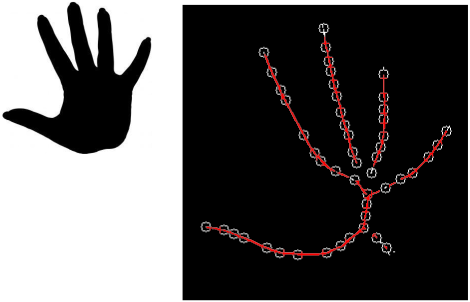
\includegraphics[width=0.4\linewidth]{./fig/features}
\caption{Ergebnis der Funktion \texttt{goodFeaturesToTrack}. Qualitätslevel: 0.1 - gewünschte Anzahl von Ecken: 50 - minimale Distanz zwischen den Ecken: 10}
\label{fig:features}
\end{figure}
Abbildung \ref{fig:features} zeigt das Ergebnis der Berechnung. Die Kreise markieren die Feature-Punkte. Wie man erkennen kann, befinden sich die Features auf der Skelettlinie. Dies ist hilfreich für die weiteren
Verbesserungen des Skeletts. Befinden sich Features außerhalb der Skelettlinien könnte die ursprüngliche Form des Skeletts und die Topologie des Objekts verfälscht werden.
\subsection{Breitensuche}
\label{subsec:breitesuche}
\begin{figure}
\centering
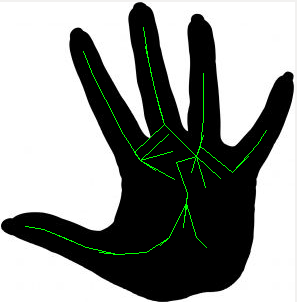
\includegraphics[width=0.4\linewidth]{./fig/hand_BFS}
\caption{Ergebnis der Breitensuche}
\label{fig:hand_BFS}
\end{figure}
\subsection{Tiefensuche}
\begin{figure}
\centering
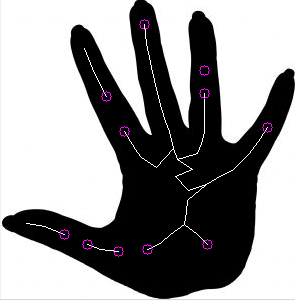
\includegraphics[width=0.4\linewidth]{./fig/hand-punkte-ohne-nachfolger}
\caption{ohne nachfolger}
\label{fig:hand-punkte-ohne-nachfolger}
\end{figure}
\label{subsec:tiefensuche}
\begin{figure}
\centering
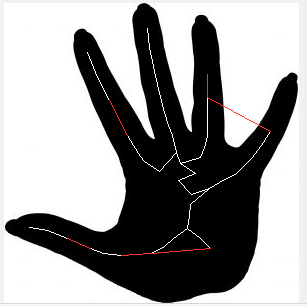
\includegraphics[width=0.4\linewidth]{./fig/hand-DFS}
\caption{Ergebnis der Tiefensuche}
\label{fig:hand-DFS}
\end{figure}